\section{}

\begin{quote}
	In summary, there is no compelling evidence to reduce the frequency of spills because of modern materials and methods. The increased corrosiveness and erosiveness of the product being transported [by the Keystone XL Pipeline] will likely cancel any gains due to materials and methods improvements and soft technological safeguards will likely become less effective over time. \citep{Stansbury2011}
\end{quote}

A graduate landing her first job in the pipeline industry in 2020 would have a very different experience than somebody who started in the year 2000. Pipeline operations are centralized in control centers. Employees control most functions of the lines on the computer, using mature software. When there are concerns about the safety of a line, rather than digging up the pipeline, the operator can send a so-called "smart pig" through it to check its condition. However, historical pipeline spill data tells a different picture. Crude oil pipelines have benefited from improved corrosion protection, but the safety performance of refined petroleum pipelines has stagnated. From the year 2000 to the year 2019, the spill volume has been consistently at a level of about 20 barrels spilled per billion barrel-miles transported (see Figure 1). Then what is all the rhetoric of technology, development, and learning from spills about?

\noindent{\hrulefill
	
\centerline{Insert Figure 1 about here}
	
\hrulefill}
\begin{figure}
	\caption{Pipeline safety improvements at the industry level}
	\centerline{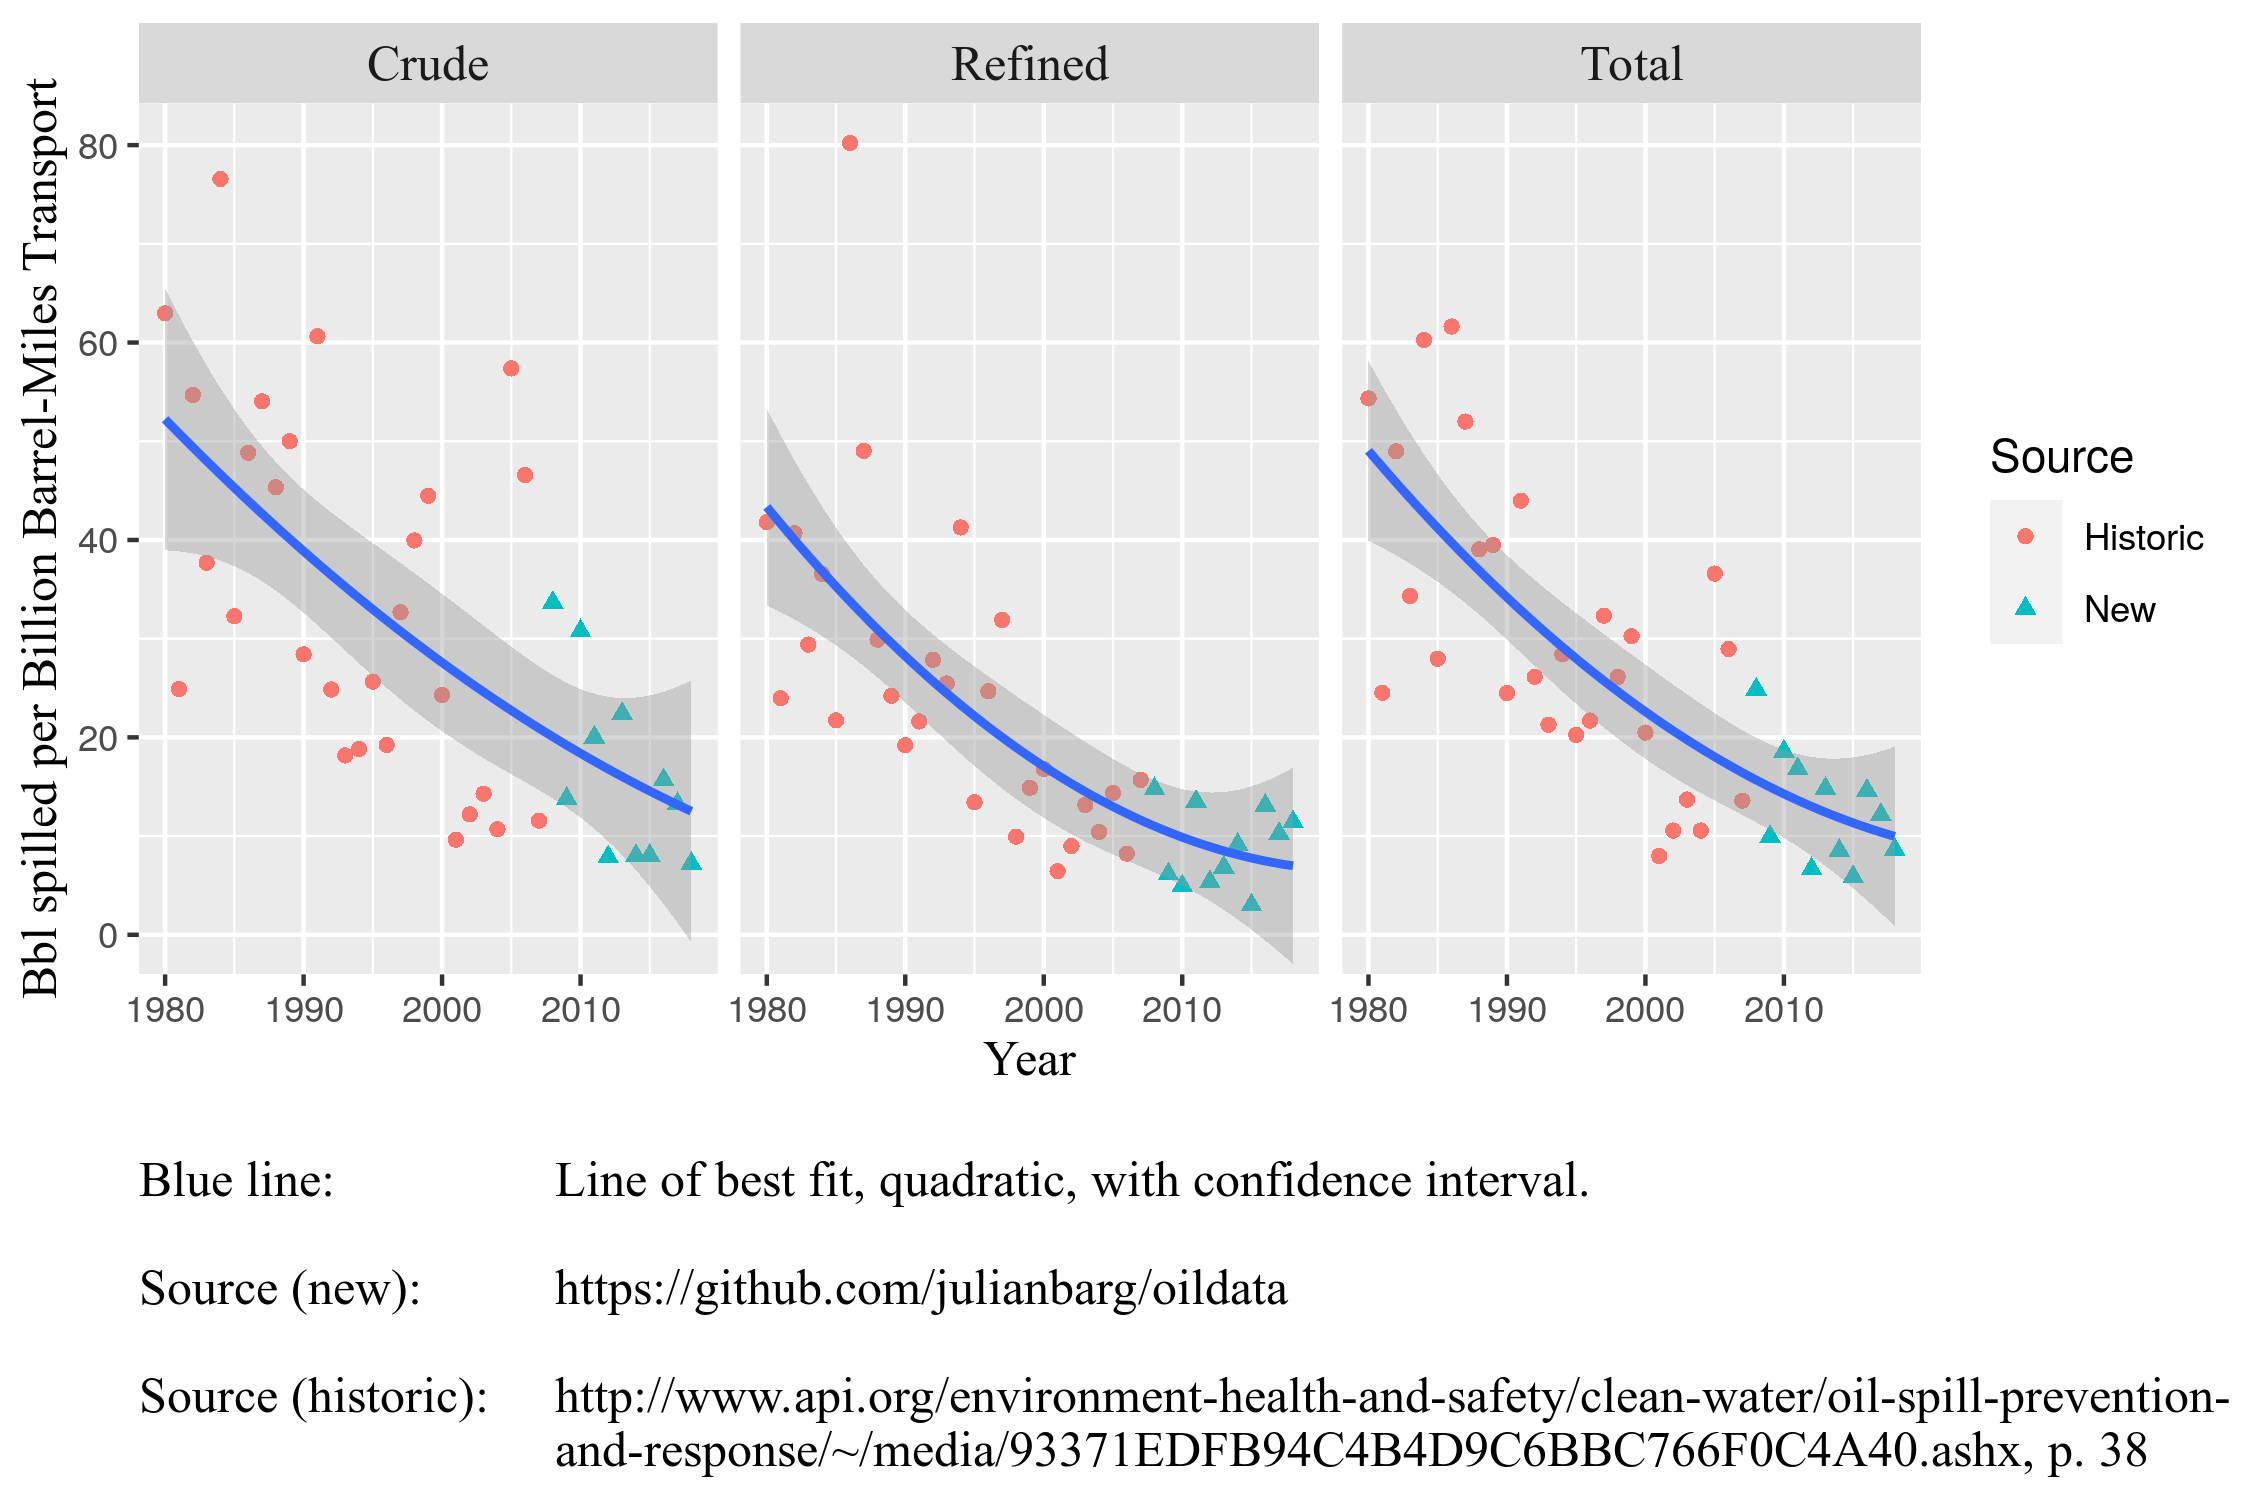
\includegraphics{../illustrations/population_learning_4.png}}
\end{figure}

This dissertation uses two lenses to analyze the phenomenon of pipeline safety: organizational learning and greenwashing. Organizational learning is a useful literature to shed light on how insights from pipeline spills affect the subsequent development of technology and routines \citep{Maslach2018}. However, the literature ceases to be useful where learning comes to halt, or where safety turns from something to be attained to something to be demonstrated to stakeholders and the regulator. Greenwashing allows us to examine this issue of deliberately misleading behavior \citep{Lyon2015}. The first chapter engages the mainstream learning literature. The second chapter summarizes the different streams of the learning literature and argues that a less technocentric view could pave a way for overcoming limits of the literature and limits to learning alike. The third chapter uses the lense of greenwashing to highlight the toxic behavior at the other end of the spectrum--intentionally misleading communication.

The first chapter of this dissertation begins with an orthodox view of organizational learning. Organizational learning is a useful frame for analyzing the technological side of pipeline safety, and why certain safety improvements are attained. Qualitative data reveals the learning processes taking place within the industry. The usefulness of an orthodox theory of organizational learning ends where we can observe that learning continues, but no more improvements in pipeline safety are achieved (Figure 1). The learning literature predicts this bottoming out \citep{Argote2013-1}, but does not address whether learning curves converge because learning stops, or for other reasons. This chapter examines the mechanisms behind safety improvements, the limits to learning, and the bottoming out of pipeline safety.

The second chapter raises the issue of validity in organizational learning \citep{Rerup2020}. The current consensus is that as organizations accumulate experience from performing a task, their performance increases \citep{Argote2011}. But, as demonstrated above, one can observe an accumulation of experience with a corresponding change in cognition--a process of organizational learning--without the accompanying change in performance. Outside the literature stream on \textit{organizational knowledge} \citep{Bingham2011}, authors emphasize the ambiguity of organizational experience \citep{March2010}. This stream would contend that sometimes, to attain success, a substantial break with precedent is necessary. This chapter reunites these two disparate streams of the organizational learning literature.
% high and low intellect, second loop learning, exploration and exploitation, competency trap

The third chapter discusses greenwashing as a reason why pipelines continue to fail. Despite March raising the issue of goals, coalitions, and politics in his early work \citep{March1963}, the topic is inexplicably absent from the current literature. Internal industry standards and company practice show that new insights are incorporated into practice. But the lived reality of incidents and spills is not what shapes communication with external stakeholders. Instead, in the classic greenwashing fashion, outside-facing documents are carefully crafted to convey an image of pipelines as safe and responsible, and catastrophic spills or near-spills not being the norm, but rare exceptions--the actors craft a public image \citep{Lyon2015}. For instance, to obtain a permit for the construction of a new pipeline, a pipeline operator has to establish that the pipeline is safe. Similarly, support from the public and state governments requires for pipelines to be perceived as safe. The third chapter discusses how technologies can be used in greenwashing attempts to give an industry a modern, and safe image.

% Paragraph on proposal structure

\subsection{Studying pipeline spills as a way to study environmental impacts}

This section lays out the motivation for studying the pipeline industry. The "gold standard" for sustainability research is to comprehensively measure environmental impacts. A common approach for doing so is to use ESG indicators. However, many barriers have to be overcome to make effective use of ESG indicators. Specifically, how the indicator is constructed has to be taken into consideration: the researcher has to be aware that the indicator is a product of social construction and has to treat it as such when conducting empirical research \citep{Eccles2019}. In particular, comparisons across industries are problematic. ESG indicators are always a combination of other metrics, and when for instance one of these metrics dominates the impact of an industry (e.g., downstream emissions of the fossil fuel industry), that should be taken into consideration during research design. Data availability also tends to be better for large corporations, favoring a cross-industry approach over intra-industry tests.

Moving from an ESG indicator to a more specific metric means making a sacrifice. The researcher to some degree forgoes the aspiration to measure impacts comprehensively, and research may become susceptible to greenwashing. For example, a chemical producer might try to improve its image by improving worker conditions; to then make any generalized statements on the sustainability of the corporation's operations without also taking into account e.g., environmental emissions would draw a wrong picture. On the flip side, to judge chemical company with excessive deaths only by its environmental impacts would also be flawed. By focusing on just one issue these complexities are lost.

The only context where focusing on just one metric would be justified is when that metric represents the most important area of impact. Coal power plants for instance are characterized by the high number of respiratory problems and indirect deaths they cause through air pollution, and the nuclear industry by its catastrophic potential. For pipelines, the case is less clear, because of their role in the fossil fuel supply chain, and by extension global climate change. However, pipelines are not indispensable for the global fossil fuel. A large share of petroleum transport globally happens by ship, which is also very cost-efficient. Thus, the pipeline industry's environmental impact is largely characterized by pipeline spills, especially because of their catastrophic potential.

Because pipeline spills dominate the pipeline industry's environmental impact, we can use the spill data to generate insights on \textit{organzational learning} and \textit{greenwashing} that should hold even if we do not take other impacts into consideration. First, we will examine the limits to \textit{organizational learning}. Individual oil spills are well documented, giving us access to the lessons to be learned from hundreds of events every year. In case of the most severe spills, where supposedly the largest amount of learning occurs \citep{Madsen2010}, the spill causes and lessons learned are further spelled out in detailed reports by the National Transportation Safety Board (NTSB). \citet{Madsen2009} carries out a similar industry-wide study of organizational learning on fatal accidents in US coal mining. Madsen uses that context to extract evidence on organization-level learning from failure. The context of the pipeline industry allows us to expand on Madsen's work and also comment on the industry-wide convergence of learning (as evident from the normalized rate of spills). Further, the nature of the outcome variable (see previous paragraph) allows for a discussion at the intersection of corporate (environmental) sustainability and organizational learning \citep{George2015}. In other words, this research allows for comments on some of the same processes that were discussed by \citet{Wright2017} with regard to climate change being picked up by corporations but insufficiently tackled, albeit from from a slightly different, quantitative perspective. This perspective recognizes changes that have been made while acknowledging that pipeline spills remain to be an important environmental issue.

\textit{Greenwashing} is the second area that pipeline spill data can shed light on. As hinted at above, greenwashing is difficult to capture because organizations are deliberately cultivating their image. Where greenwashing takes the shape of decoupling between internal action and communication with the environment \citep{Lyon2015}, ESG indicators are also affected. Pipeline operators can misrepresent their efforts to improve pipeline safety, but pipeline spills are generally well documented. I probably don't have to remind the reader that oil in its crude form is a black, gooey substance. On waterways, refined oil forms distinct films. Both crude and refined oil give off a distinct odor. Pipeline spills are often initially discovered by residents. Emergency responders and specialized spill response staff as well as often journalists are all groups of people that would become aware of pipelines spills once they reach a certain scale. In short there are many reasons why pipeline spills are better documented than e.g., human rights violations or greenhouse gas emissions. For these reasons, we can identify well for the pipeline industry the organizations that communicate a commitment to pipeline safety but exhibit a poor safety performance. Because the datasets are longitudinal in nature and cover (at least for pipeline miles and spills) the complete industry, it offers an opportunity to study the scope of greenwashing in an industry as well as its development over time.

As shown in this section, examining the pipeline industry provides a range of insights. These insights both take the form of contributions to theory development, and also allow us to take stock of an industry and its development over time. The second form of insight could become relevant for stakeholders, such as NGOs that monitor the pipeline or other industries. Real-world oriented questions that this research could shed light on are "what should stakeholders expect of polluting industries both in terms of cleanup and greenwashing?" Other questions, this research cannot answer, but give an impetus for an informed debate, e.g., "what level of spills is acceptable, and how do we get there?" Finally, while the fact that pipeline spills dominate the pipeline industry's environmental impacts is convenient for research, it may also represent a limitation. The complexity of managing multiple impacts at once compared to focusing only on one impact means that there might be different dynamics at play in the context of the pipeline industry compared to other, more complex industries.